%14.06  - 21.06:
%5. Evaluation => ca. 15 Seiten
%- Trainingsdaten (welche woher kommen die, wie sehen die Systeme aus...)
%- Genauigkeit der Lösung (K-Cross-validation)
%- Betrachtung der Regeln (Bäume malen)
%- Verhalten bei weniger Trainingsdaten (Inverse Cross-Valdiation).
%- Leistungsverhalten des Machine LEarnings (Wieviel Performance kostet das)

\section{Auswertung}

\subsection{Daten}


Die Experimente wurden auf einem Cluster mit 20 Knoten durchgeführt.
10 E/A-Knoten sind jeweils mit einem Intel Xeon E3-1278@3.4 GHz, 16 GByte RAM und einer Seagate Barracude 7200.12 ausgestattet.
Die Knoten sind mit einem Gigabit Ethernet miteinander verbunden und die Leistung einer HDD ist ca. 100 MiB/s.
Die E/A-Knoten laufen mit CentOS 6.5 und Lustre 2.5.

In dem Experiment wurden 20 verschiedenen Datengrößen ausgeführt.
10 davon sind Potenzen zu Basis 2 ($size_{i+1} = size_i * 4$) und 10 sind keine ($size_{i+1} = size_i * 4 + 1$), mit $size_0 = 1$ und $0 \leq i < 10$.
Pro Datengröße wurden 10000 Messungen gemacht und der Wert gemittelt.
Der Experiment wurde einmal für Leseoperationen und einmal für Schreiboperationen durchgeführt.
Während der Messungen wurden alle weiteren Prozesse auf das minimum beschränkt, vor allem liefen keine weiteren E/A-intensiven Benutzerprozesse.
Der Graph in der \figref{fig:eva:origperf} zeigt die Durchsatzwerte der Messreihe.

% Read Sizes
%1, 4, 16, 64, 256, 1024, 4096, 16384, 65536, 262144
%2, 5, 17, 65, 257, 1025, 4097, 16385, 65537, 262145

% Write Size
%1, 4, 16, 64, 256, 1024, 4096, 16384, 65536, 262144, 
%2, 5, 17, 65, 257, 1025, 4097, 16385, 65537, 262145

%#AbsTime,DeltaTime,fd,OpTyp,DeltaOffset,Size,Duration 

\begin{figure}[ht]
	\hfill
	\subfigure[Leseoperationen.]{
		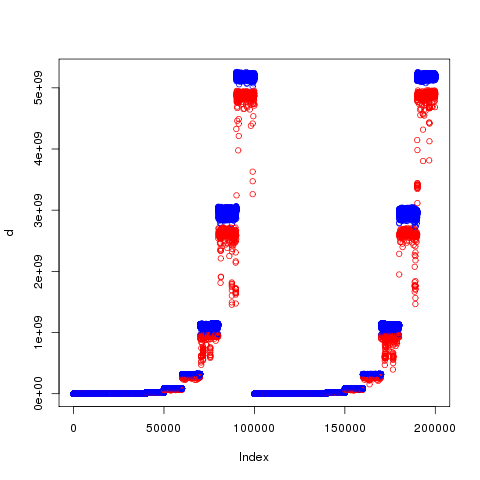
\includegraphics[width=.47\textwidth]{pictures/OriginalPerfR.png}
		\label{fig:eva:origperfr}
	}
	\hfill
	\subfigure[Schreiboperationen.]{
		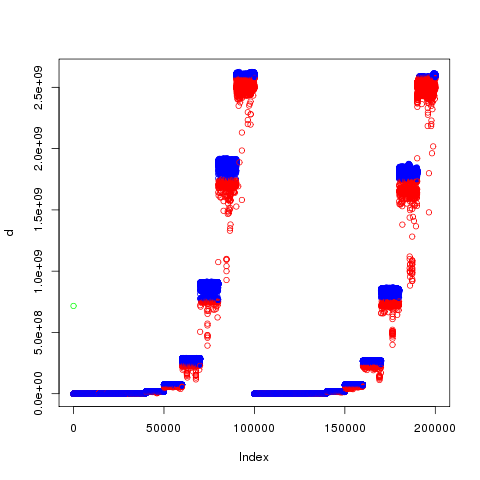
\includegraphics[width=.47\textwidth]{pictures/OriginalPerfW.png}
		\label{fig:eva:origperfw}
	}
	\hfill
	\caption{Durchsatz von Operation mit verschiedenen Datengrößen. Die ersten 100000 Werte gehöhren zu den Datengrößen, die eine Potenz zu Basis 2 sind und die restlichen 100000 Werte gehöhren zu den, die es nicht sind.}
	\label{fig:eva:origperf}
\end{figure}

In einem idealen System ohne Systemaufruf-Overhead würde die Verarbeitung von einem Byte die gleiche Zeit dauern, wenn die Operation an der gleichen Cacheebene stattgefunden hätte.
Die Messung zeigt aber  also die Zeit pro Operation an einem Byte, so sieht man, dass die Zeit bei kleinen Datengrößen wesentlich größer ist.
Das kommt von dem Overhead von den Operationen.

Man schon an dieser Stelle vermuten, dass der systematische Fehler, wenn man ihn nicht eliminiert, sich in der Baumgröße niederschlagen wird und die Auswertung erschwert.

\begin{figure}[ht]
	\hfill
	\subfigure[Leseoperationen.]{
		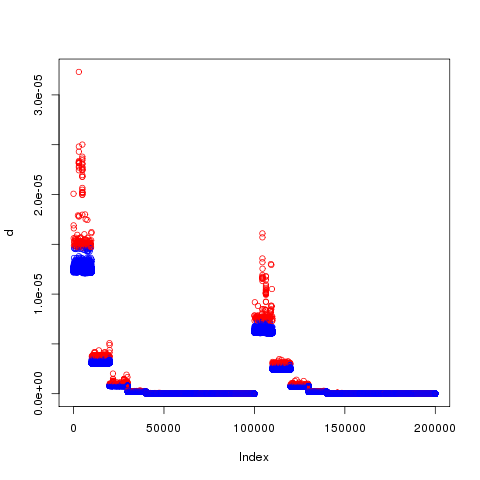
\includegraphics[width=.47\textwidth]{pictures/OriginalRPerfR.png}
		\label{fig:eva:origrperfr}
	}
	\hfill
	\subfigure[Schreiboperationen.]{
		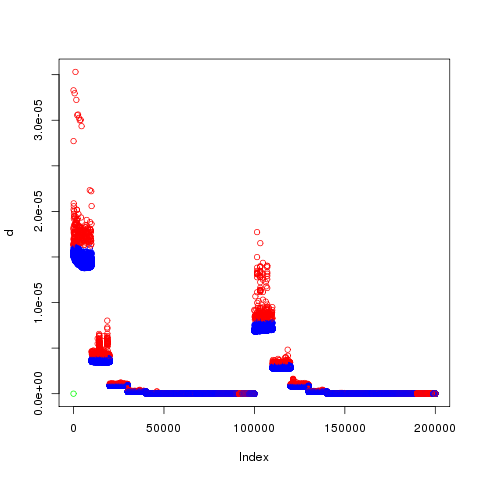
\includegraphics[width=.47\textwidth]{pictures/OriginalRPerfW.png}
		\label{fig:eva:origrperfw}
	}
	\hfill
	\caption{Zeit für die Verarbeitung eines Bytes.}
	\label{fig:eva:origrperf}
\end{figure}


Die Daten sind bereits bereits mit 11 Gruppen bewertet.


%label
%cached CPU      : 379472
%cached memory   : 20527
%fast I/O        : 1
%unexpected slow : 1
%unknown         : 0
%discarded       : 0
%(Other)         : 0
%- unknown
%- discarded
%- cached CPU
%- cached memory
%- cached storage
%- fast I/O
%- normal I/O
%- slow I/O
%- unexpected fast
%- unexpected between
%- unexpected slow
\begin{table}
	\centering
	\begin{tabular}{l|llll}
		Typ                    & min & average & max & size \\
		\hline
		unbekannt              &     &         &     & 0\\
		verworfen              &     &         &     & 0\\
		cached CPU             &     &         &     & 379472\\
		cached Arbeitsspeicher &     &         &     & 20527\\
		cached Massenspeicher  &     &         &     & 0\\
		schnelle E/A           &     &         &     & 1\\
		normale E/A            &     &         &     & -\\
		langsame E/A           &     &         &     & -\\
		unerwartet schnell     &     &         &     & -\\
		unerwartet normal      &     &         &     & -\\
		unerwartet langsam     &     &         &     & 1 
	\end{tabular}
	\caption{Verteilung der Daten für Lese- und Schreiboperationen.}
\end{table}

\subsection{Leistungsvorhersage}

Mit dem Leistungsprädiktor wurde ein Entscheidungsbaum trainiert.
Als Features wurden benutzt die Datengröße, Operationsdauer und Offset zwischen den Operationen.
Als Label wurde die Leistungswerte benutzt.
Um die Komplexität zu reduzieren, wurde der Baumtiefe auf 4 Ebenen beschränkt.

Um die Leistung vorherzusagen, müssen zuerst Annahmen getroffen über die Größen, die einen Einfluss auf die Leistung haben und dann in die Features umgesetzt werden.
In diesem Experiment, wird von zwei Annahmen ausgegagen:
1. Die Datengröße hat einen direkten Einfluss auf die Leistung.
Wenn die Daten in den Cache passen, dann können wir eine hohe Leistung erwarten.
2. Wenn vorheriger Zugriff schnell war, dann ist die Wahrscheinlichkeit hoch, dass auch der nächster Zugriff hoch sein wird.


\begin{figure}[ht]
	\centering
	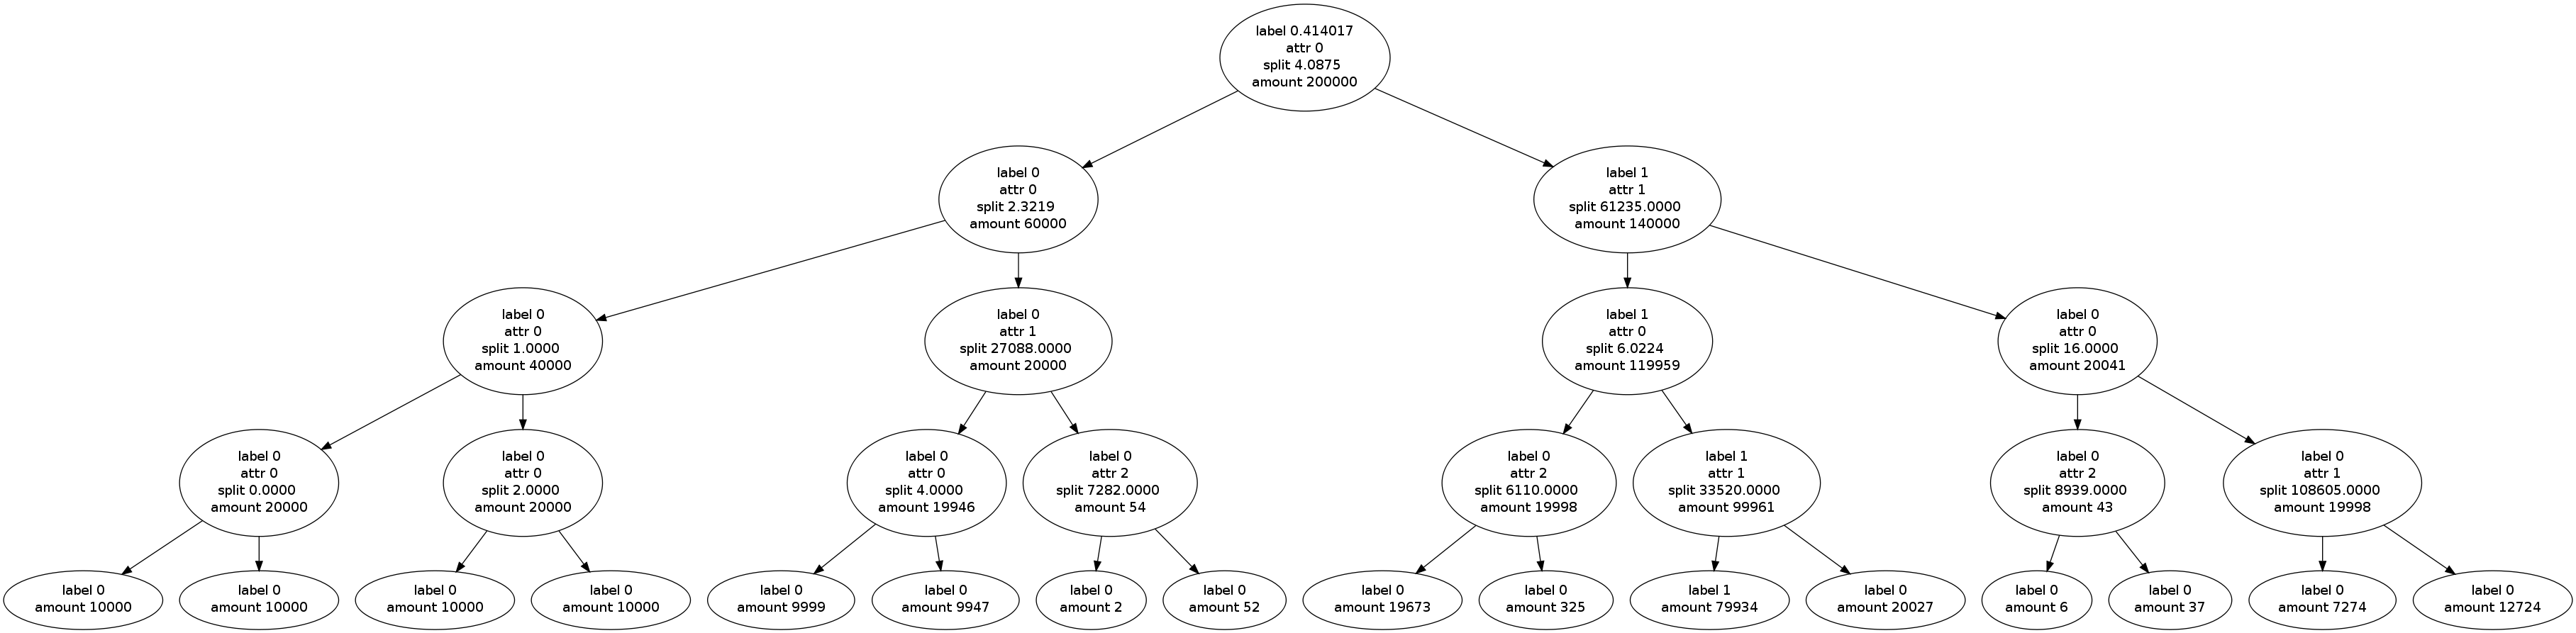
\includegraphics[width=\textwidth]{pictures/predictor.png}
	\caption{Entscheidungsbaum für die Leistungvorhersage.}
	\label{fig:eva:predTree}
\end{figure}

Zum Auswerten der Vorhersage wird bei der Kreuzvalidierung die mittlere quadratische Abweichung verwendet.
Der Wert ist zwar recht gross.
Das zeigt einerseits, dass die Features alleine nicht ausreichen, um die Leistung präzise vorherzusagen, aber er zeigt auch, dass die Features für die Leistungsvorhersage relevant sind.


Die Leistungsvorhersage anhand von diesen Kriterien klappt mit ausreichend großen Bäumen recht gut.
Mit einem Baum mit der Tiefe 8 ist die mittlere quadratische Abweichung $\sigma = 0.000135486$.


\subsection{Klassifizierung nach Leistung}

Der Leistungswert der Aktivität dient als ein Feature.
Er lässt sich aus der Datengröße und der Operationsdauer berechnen, also $f_1 = size / duration$.
Das zweite Feature wird direkt aus dem ersten mit der Formel $f_2 = log2(f_1) \cdot max(f_1)$ berechnet.
Damit lassen sich die kleinen Stufen betonen und werden somit von dem Lernalgorithmus wargenommen.
Die Abbildung \todo{Refezenz zum Graphen} schaut so aus.

\begin{figure}[ht]
	\hfill
	\subfigure[$f_1 = p$]{
		\missingfigure[figwidth=.46\textwidth]{p}
		%\includegraphics[width=.47\textwidth]{pictures/Read-Perf.png}
		\label{fig:eva:readperf}
	}
	\hfill
	\subfigure[$f_2 = log2(p) \cdot max(f_1)$]{
		\missingfigure[figwidth=.46\textwidth]{log2(p)}
		%\includegraphics[width=.47\textwidth]{pictures/Read-PerfLog2.png}
		\label{fig:eva:readperflog2}
	}
	\hfill
	\caption{Features $f_1$ und $f_2$ sortiert in aufsteigender Reihenfolge.}
	\label{fig:eva:transfeats}
\end{figure}



